\documentclass[usenames,dvipsnames,aspectratio=169]{beamer}
\usepackage{../common/prgBasics}

\title[Lecture 9.]{Programming basics}
\subtitle{(GKNB\_INTA023)}

\begin{document}

%1
\begin{frame}[plain]
  \titlepage
\end{frame}

%2
\begin{frame}{Sorting numbers}
  Task:
  \begin{itemize}
    \item Improve the existing bubble sort program! Let the user enter the numbers to be sorted! Finish reading the input by entering a negative number.
    \item Entering more numbers than the size of the array must be prevented.
  \end{itemize}
  Problems:
  \begin{itemize}
    \item The count of numbers should be known at compile time
    \item Undersized array $\to$ there will be no space for the data
    \item Oversized array $\to$ wasting the memory
    \item The oversized array causes the smaller problem.
  \end{itemize}
\end{frame}

%3
\begin{frame}[fragile]{Sorting numbers}
  \begin{columns}[T]
    \column{.45\textwidth}
      \begin{block}{Output1}
        \small
        \begin{verbatim}
Enter non-negative numbers
Number #1: 2
Number #2: 4
Number #3: 1
Number #4: 3
Number #5: -1
After sorting:
1       2       3       4    
\end{verbatim}
      \end{block}
    \column{.45\textwidth}
      \begin{block}{Output2}
        \small
        \begin{verbatim}
Enter non-negative numbers
Number #1: 5
Number #2: 4
Number #3: 3
Number #4: 2
Number #5: 1
After sorting:
1       2       3       4       5    
\end{verbatim}
      \end{block}
  \end{columns}
\end{frame}

%4
\begin{frame}{Sorting numbers}
  \begin{exampleblock}{\textattachfile{bubble5.c}{bubble5.c}}
    \lstinputlisting[style=c,linerange={3-3},numbers=left,firstnumber=3]{bubble5.c}
    \lstinputlisting[style=c,linerange={37-46},numbers=left,firstnumber=37]{bubble5.c}
  \end{exampleblock}
\end{frame}

%5
\begin{frame}{Sorting numbers}
  \begin{exampleblock}{\textattachfile{bubble5.c}{bubble5.c}}
    \lstinputlisting[style=c,linerange={5-16},numbers=left,firstnumber=5]{bubble5.c}
  \end{exampleblock}
\end{frame}

%6
\begin{frame}{Dynamic memory allocation}
  \begin{itemize}
    \small
    \item The programmer decides the lifetime of dynamic variables
    \item \texttt{stdlib.h} must be included
    \item Memory allocation:\\
      \begin{itemize}
        \item \texttt{void *malloc(size\_t size);} \\
          Allocates \texttt{size} bytes of memory and returns its address. The allocated area is \emph{uninitialized}.
        \item \texttt{void *calloc(size\_t nmemb, size\_t size);} \\
          Allocates and returns the address of a continuous memory area for an array containing \texttt{nmemb} elements, each of which requires \texttt{size} bytes of memory. The area is \emph{initialized to zeros}.
        \item \texttt{void *realloc(void *ptr, size\_t size);} \\
          Resizing the already allocated memory area without modifying the stored content.
      \end{itemize}
    \item The return value is NULL in case of an error $\to$ should be checked
    \item Freeing memory: \texttt{void free(void *ptr);}
    \item The same meory area cannot be freed several times
    \item Freeing NULL does not cause problems
  \end{itemize}
\end{frame}

%7
\begin{frame}{Sorting numbers}
  Tasks:
  \begin{itemize}
    \item Allocate memory dynamically for the array containing the numbers to be sorted
    \item Enter the count of numbers first, then allocate the required amount of memory and read the numbers
    \item Do not forget to free the allocated area as soon as possible
  \end{itemize}
\end{frame}

%8
\begin{frame}{Sorting numbers}
  \begin{exampleblock}{\textattachfile{bubble6.c}{bubble6.c}}
    \lstinputlisting[style=c,linerange={34-42},firstnumber=34]{bubble6.c}
  \end{exampleblock}
\end{frame}

%9
\begin{frame}{Sorting numbers}
  \footnotesize
  \begin{exampleblock}{\textattachfile{bubble6.c}{bubble6.c}}
    \lstinputlisting[style=c,linerange={4-13},firstnumber=4]{bubble6.c}
  \end{exampleblock}
\end{frame}

%10
\begin{frame}{Student register}
  Tasks:
  \begin{itemize}
    \item Record the names and grades of students (one grade per student)
    \item Read the number of students first, then allocate the required amount of memory to store an array of name-grade structures
    \item Allocate memory dynamically even for the names!
    \item Sort the list according to the names and display it
  \end{itemize}
\end{frame}

% %11
% \begin{frame}{Hallgatói nyilvántartás}
%   \footnotesize
%   \begin{exampleblock}{\textattachfile{hallgatok1.c}{hallgatok1.c}}
%     \lstinputlisting[style=c,linerange={6-9},numbers=left,firstnumber=6]{hallgatok1.c}
%     \lstinputlisting[style=c,linerange={72-81},numbers=left,firstnumber=72]{hallgatok1.c}
%   \end{exampleblock}
% \end{frame}

% %12
% \begin{frame}{Hallgatói nyilvántartás}
%   \scriptsize
%   \begin{exampleblock}{\textattachfile{hallgatok1.c}{hallgatok1.c}}
%     \lstinputlisting[style=c,linerange={20-38},numbers=left,firstnumber=20]{hallgatok1.c}
%   \end{exampleblock}
% \end{frame}

% %13
% \begin{frame}{Hallgatói nyilvántartás}
%   \begin{exampleblock}{\textattachfile{hallgatok1.c}{hallgatok1.c}}
%     \lstinputlisting[style=c,linerange={40-50},numbers=left,firstnumber=40]{hallgatok1.c}
%   \end{exampleblock}
% \end{frame}

% %14
% \begin{frame}{Hallgatói nyilvántartás}
%   \footnotesize
%   \begin{exampleblock}{\textattachfile{hallgatok1.c}{hallgatok1.c}}
%     \lstinputlisting[style=c,linerange={52-63},numbers=left,firstnumber=52]{hallgatok1.c}
%   \end{exampleblock}
% \end{frame}

% %15
% \begin{frame}{Hallgatói nyilvántartás}
%   \begin{exampleblock}{\textattachfile{hallgatok1.c}{hallgatok1.c}}
%     \lstinputlisting[style=c,linerange={65-70},numbers=left,firstnumber=65]{hallgatok1.c}
%   \end{exampleblock}
% \end{frame}

% %16
% \begin{frame}{Számok rendezése}
%   \small
%   Feladat:
%   \begin{itemize}
%     \item Tegyük még kényelmesebbé a korábbi, számokat rendező programunk használatát azzal, hogy a felhasználónak ne kelljen 
% előre összeszámolnia, hány adatot kell rendeznie!
%     \item Jelezze valamilyen speciális érték az adatbevitel végét! $\to$ negatív érték
%   \end{itemize}
%   Probléma:
%   \begin{itemize}
%     \item[] Mekkora területet foglaljunk, ha azt sem tudjuk, hány adatot kell tárolni?
%   \end{itemize}
%   Megoldás:
%   \begin{itemize}
%     \item[] Lefoglalunk egy kis memóriablokkot, majd ha ez elfogy, mindig megduplázzuk annak méretét.
%   \end{itemize}
%   Megjegyzés:
%   \begin{itemize}
%     \item[] Az egyszerűség és tömörség kedvéért a továbbiakban feltételezzük a memóriafoglalások sikerességét.
%   \end{itemize}
% \end{frame}

% %17
% \begin{frame}{Számok rendezése}
%   \begin{exampleblock}{\textattachfile{buborek7.c}{buborek7.c}}
%     \lstinputlisting[style=c,linerange={45-55},numbers=left,firstnumber=45]{buborek7.c}
%   \end{exampleblock}
% \end{frame}

% %18
% \begin{frame}{Számok rendezése}
%   \fontsize{8}{9} \selectfont
%   \begin{exampleblock}{\textattachfile{buborek7.c}{buborek7.c}}
%     \lstinputlisting[style=c,linerange={4-24},numbers=left,firstnumber=4]{buborek7.c}
%   \end{exampleblock}
% \end{frame}

% %19
% \begin{frame}[fragile]{Számok rendezése}
%   \fontsize{7}{8} \selectfont
%   \begin{block}{Kimenet}
%     \begin{verbatim}
% Adjon meg nemnegativ szamokat!
%         [Felhasznalva: 0, tombelemek szama: 1]
% 1. szam: 7
%         [Felhasznalva: 1, tombelemek szama: 1]
% 2. szam: 1
%         [Memoriafoglalas]
%         [Felhasznalva: 2, tombelemek szama: 2]
% 3. szam: 9
%         [Memoriafoglalas]
%         [Felhasznalva: 3, tombelemek szama: 4]
% 4. szam: 11
%         [Felhasznalva: 4, tombelemek szama: 4]
% 5. szam: 21
%         [Memoriafoglalas]
%         [Felhasznalva: 5, tombelemek szama: 8]
% 6. szam: 67
%         [Felhasznalva: 6, tombelemek szama: 8]
% 7. szam: 22
%         [Felhasznalva: 7, tombelemek szama: 8]
% 8. szam: 42
%         [Felhasznalva: 8, tombelemek szama: 8]
% 9. szam: -1
% Rendezes utan:
% 1       7       9       11      21      22      42      67
% \end{verbatim}
%   \end{block}
% \end{frame}

% %20
% \begin{frame}{Téglalapok rajzolása}
%   Feladat:
%   \begin{itemize}
%     \item Alakítsuk át a téglalap rajzoló programot is hasonlóan, de most mindig ugyanannyival növeljük a tömb méretét, ha 
% elfogy a hely!
%     \item A tömböt lefoglaló és feltöltő függvény adja vissza az elemek számát, a tömb címét pedig írja a paraméterként kapott 
% címre!
%   \end{itemize}
%   \begin{exampleblock}{\textattachfile{teglalap3.c}{teglalap3.c}}
%     \scriptsize
%     \lstinputlisting[style=c,linerange={90-97},numbers=left,firstnumber=90]{teglalap3.c}
%   \end{exampleblock}
% \end{frame}

% %21
% \begin{frame}{Téglalapok rajzolása}
%   \begin{exampleblock}{\textattachfile{teglalap3.c}{teglalap3.c}}
%     \footnotesize
%     \lstinputlisting[style=c,linerange={59-74},numbers=left,firstnumber=59]{teglalap3.c}
%   \end{exampleblock}
% \end{frame}

% %22
% \begin{frame}{Téglalapok rajzolása}
%   \begin{exampleblock}{\textattachfile{teglalap3.c}{teglalap3.c}}
%     \footnotesize
%     \lstinputlisting[style=c,linerange={75-88},numbers=left,firstnumber=75]{teglalap3.c}
%   \end{exampleblock}
% \end{frame}

% %23
% \begin{frame}[fragile]{Téglalapok rajzolása}
%   \begin{columns}[T]
%     \column{0.6\textwidth}
%       \begin{block}{Kimenet 1/2}
%         \tiny
%         \begin{verbatim}
% Rajzprogram - adja meg a téglalapok adatait!
%         [Felhasznalva: 0, elemszam: 2]
% 1. teglalap BF sarok X: [0, 78] (negativra vege) 3
% 1. teglalap BF sarok Y: [0, 23] 3
% 1. teglalap JA sarok X: [4, 79] 6
% 1. teglalap JA sarok Y: [4, 24] 6
% 1. teglalap rajzoló karaktere: +
%         [Felhasznalva: 1, elemszam: 2]
% 2. teglalap BF sarok X: [0, 78] (negativra vege) 5
% 2. teglalap BF sarok Y: [0, 23] 5
% 2. teglalap JA sarok X: [6, 79] 8
% 2. teglalap JA sarok Y: [6, 24] 8
% 2. teglalap rajzoló karaktere: -
%         [Felhasznalva: 2, elemszam: 2]
% 3. teglalap BF sarok X: [0, 78] (negativra vege) 7
%         [Memoriafoglalas]
% 3. teglalap BF sarok Y: [0, 23] 7
% 3. teglalap JA sarok X: [8, 79] 10
% 3. teglalap JA sarok Y: [8, 24] 10
% 3. teglalap rajzoló karaktere: *
%         [Felhasznalva: 3, elemszam: 4]
% 4. teglalap BF sarok X: [0, 78] (negativra vege) -1
% \end{verbatim}
%       \end{block}
%     \column{0.4\textwidth}
%       \begin{block}{Kimenet 2/2}
%         \begin{verbatim}
%    ++++                                                                         
%    ++++                                                                         
%    ++----                                                                       
%    ++----                                                                       
%      --****                                                                     
%      --****                                                                     
%        ****                                                                     
%        ****
% \end{verbatim}
%       \end{block}
%   \end{columns}
% \end{frame}

% %24
% \begin{frame}{Mátrixok}
%   Mátrix: azonos típusú elemek kétdimenziós tömbje\\
%   A C-ben csak egydimenziós tömbök léteznek, de ezeket tetszőleges mélységben egymásba lehet ágyazni! $\to$ \\
%   \qquad mátrix = vektorokból álló vektor\\
%   \begin{columns}[T]
%     \column{0.5\textwidth}
%       \hspace{.25cm} $A = \left[ \begin{array}{cccc}
%                      11 & 12 & 13 & 14 \\
%                      21 & 22 & 23 & 24 \\
%                      31 & 32 & 33 & 34 \\
%                    \end{array}
%                 \right]$
%     \column{0.5\textwidth}
%       \texttt{int A[3][4] = \{ \\
%       \qquad \{11, 12, 13, 14\},\\
%       \qquad \{21, 22, 23, 24\},\\
%       \qquad \{31, 32, 33, 34\} \};}
%   \end{columns}
%   \begin{center}
%     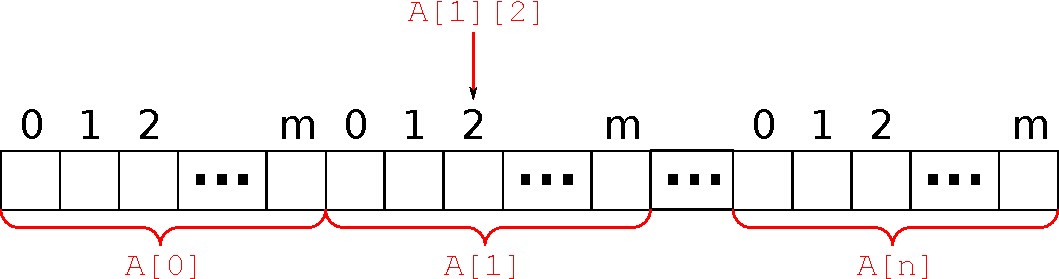
\includegraphics[width=0.85\textwidth]{matrix.pdf}
%   \end{center}
%   Mátrixok összeadása: $(A+B)[i,j] = A[i,j] + B[i,j]$, ahol $A$ és $B$ két $n\times m$ méretű mátrix.\\
% \end{frame}

% %25
% \begin{frame}{Mátrixok}
%   \begin{exampleblock}{\textattachfile{mtxOsszead1.c}{mtxOsszead1.c}}
%     \scriptsize
%     \lstinputlisting[style=c,linerange={4-20},numbers=left,firstnumber=4]{mtxOsszead1.c}
%   \end{exampleblock}
% \end{frame}

% %26
% \begin{frame}{Mátrixok}
%   \scriptsize
%   \begin{exampleblock}{\textattachfile{mtxOsszead1.c}{mtxOsszead1.c}}
%     \scriptsize
%     \lstinputlisting[style=c,linerange={21-40},numbers=left,firstnumber=21]{mtxOsszead1.c}
%   \end{exampleblock}
% \end{frame}

% %27
% \begin{frame}[fragile]{Mátrixok}
%   \begin{block}{Kimenet}
%     \begin{verbatim}
% 11 12 13 14   33 49 36 12   44 61 49 26 
% 21 22 23 24 + 20 45 24 18 = 41 67 47 42 
% 31 32 33 34   19 10 11 42   50 42 44 76
% \end{verbatim}
%   \end{block}
%   \vfill
%   Hogyan adható át egy mátrix függvénynek?\\
%   \begin{exampleblock}{OK \checkmark}
%     \texttt{void fv(int t[SOROK][OSZLOPOK]) \{ //...\\
%     void fv(int t[][OSZLOPOK]) \{ //...\\
%     void fv(int (*t)[OSZLOPOK]) \{ //...}
%   \end{exampleblock}
%   \begin{alertblock}{Hiba X -- Ez mutatótömb, nem mátrix!}
%     \texttt{void fv(int *t[OSZLOPOK]) \{ //...}
%   \end{alertblock}
% \end{frame}

% %28
% \begin{frame}{Mátrixok}
%   \begin{exampleblock}{\textattachfile{mtxOsszead2.c}{mtxOsszead2.c}}
%     \lstinputlisting[style=c,linerange={44-56},numbers=left,firstnumber=44]{mtxOsszead2.c}
%   \end{exampleblock}
% \end{frame}

% %29
% \begin{frame}{Mátrixok}
%   \scriptsize
%   \begin{exampleblock}{\textattachfile{mtxOsszead2.c}{mtxOsszead2.c}}
%     \scriptsize
%     \lstinputlisting[style=c,linerange={4-23},numbers=left,firstnumber=4]{mtxOsszead2.c}
%   \end{exampleblock}
% \end{frame}

% %30
% \begin{frame}{Mátrixok}
%   \scriptsize
%   \begin{exampleblock}{\textattachfile{mtxOsszead2.c}{mtxOsszead2.c}}
%     \scriptsize
%     \lstinputlisting[style=c,linerange={25-42},numbers=left,firstnumber=25]{mtxOsszead2.c}
%   \end{exampleblock}
% \end{frame}

% %31
% \begin{frame}{Mátrixok}
%   \begin{columns}[T]
%     \column{.5\textwidth}
%       Probléma:
%       \begin{itemize}
%         \item[] rugalmatlan függvények, mert az oszlopok száma rögzített
%       \end{itemize}
%       \vfill
%       Megoldás:
%       \begin{itemize}
%         \item hozzunk létre dinamikusan vektorokat (pl. \texttt{int*}-gal címezhetők), majd 
%         \item ezek címeit tároljuk egy újabb, dinamikus vektorban (\texttt{int**}, mutatótömb)!
%       \end{itemize}
%     \column{.5\textwidth}
%       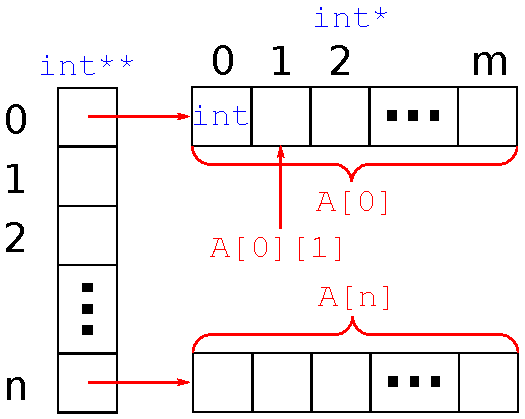
\includegraphics[width=\textwidth]{matrix2.pdf}
%   \end{columns}
% \end{frame}

% %32
% \begin{frame}{Mátrixok}
%   \footnotesize
%   \begin{exampleblock}{\textattachfile{mtxOsszead3.c}{mtxOsszead3.c}}
%     \lstinputlisting[style=c,linerange={55-70},numbers=left,firstnumber=55]{mtxOsszead3.c}
%   \end{exampleblock}
% \end{frame}

% %33
% \begin{frame}{Mátrixok}
%   \begin{exampleblock}{\textattachfile{mtxOsszead3.c}{mtxOsszead3.c}}
%     \footnotesize
%     \lstinputlisting[style=c,linerange={5-19},numbers=left,firstnumber=5]{mtxOsszead3.c}
%   \end{exampleblock}
% \end{frame}

% %34
% \begin{frame}{Mátrixok}
%   \begin{exampleblock}{\textattachfile{mtxOsszead3.c}{mtxOsszead3.c}}
%     \footnotesize
%     \lstinputlisting[style=c,linerange={21-28},numbers=left,firstnumber=21]{mtxOsszead3.c}
%     \lstinputlisting[style=c,linerange={48-53},numbers=left,firstnumber=49]{mtxOsszead3.c}
%   \end{exampleblock}
% \end{frame}

% %35
% \begin{frame}{Mátrixok}
%   Alternatív megoldás:
%   \begin{itemize}
%     \item utánozzuk a ``statikus'' tömbök memóriabeli szerkezetét, azaz
%     \item valójában vektornak foglalunk helyet, és erre képezzük le a mátrix elemeit
%   \end{itemize}
%   \begin{center}
%     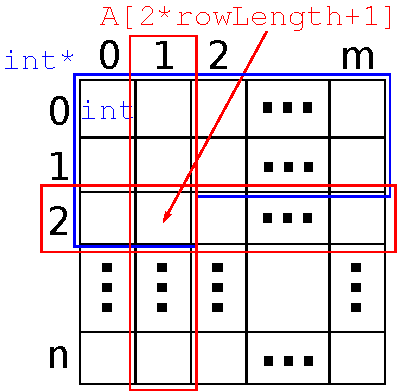
\includegraphics[scale=0.6]{matrix3.pdf}
%   \end{center}
% \end{frame}

% %36
% \begin{frame}{Mátrixok}
%   \footnotesize
%   \begin{exampleblock}{\textattachfile{mtxOsszead4.c}{mtxOsszead4.c}}
%     \lstinputlisting[style=c,linerange={44-59},numbers=left,firstnumber=44]{mtxOsszead4.c}
%   \end{exampleblock}
% \end{frame}

% %37
% \begin{frame}{Mátrixok}
%   \scriptsize
%   \begin{exampleblock}{\textattachfile{mtxOsszead4.c}{mtxOsszead4.c}}
%     \lstinputlisting[style=c,linerange={5-24},numbers=left,firstnumber=5]{mtxOsszead4.c}
%   \end{exampleblock}
% \end{frame}

\end{document}
